\chapter{Theory}

\cite{goodman2000,goodman2007,agarwal2013,classen2017,cowley1995,born1980,trigg2005,attwood1999,griffiths2005,agarwal2013,classen2017,loudon2000,mandel1995,hanburry1956,galuber2006,baym1997,zernike1938,rosen96,yabashi2002,singer2013,santra2009,krause1979,trost2020,inoue2019,sorum1987,lajunen04,mpccd,tono2013}




\paragraph{Stationarity and Ergodicity}
A process $f(t)$ is wide-sense stationary, if the expectation value $E[f(t)]$ is independent of the time $t$ and $E[f(t_1)f(t_2)]$ depends only on the time difference $\tau=f_1-f_2$. A process, for which the time average and the ensemble average are equal is called ergodic. Stationarity is a necessity for ergodicity.

random process
ergodic: time average equals expectation value
stationary: shifting all time instants by $\tau$ does not change the statistical description of the random process 



\section{Coherence}


Coherence


Spherical waves as  solutions to scalar wave equation in spherical coordinates,
\begin{equation}
	E(\vec{r},t)=E_0(k,t) \frac{e^{i\vec{r}\vec{k}-iwt}}{R}
	\end{equation}
describe light propagating isotropically. 
Superposition principle of two waves with the real amplitudes $A_{1,2}$ and phases $\phi{1,2}$
\begin{equation}
E(\vec{r},t)=E_1(\vec{r},t)+E_2\vec{r},t)=A_1*e^{i\phi_1} * e^{i\vec{r}\vec{k_1}-iw_1t} + A_1*e^{i\phi_1} * e^{i\vec{r}\vec{k_2}-iw_2t} 
\end{equation} 

The measured Intensity with measurement time $T\gg1/w$ will be
\begin{equation}
	I(\vec{r},t)\propto \int_0^T \left|E(\vec{r},t)\right|^2 \diff t .
\end{equation}

The superposition of two monochromatic, stationary waves with a fixed phase difference $\Delta \phi$, such as a wave and its time delayed copy (\fref{fig:michelson}) in a Michelson interferometer, gives rise to interference fringes
\begin{equation}
	\left<I(\vec{r},t)\right>=I_1+I_2+2\sqrt{I_1I_2}\cos\left((\vec{k_1}-\vec{k_2})\vec{r}+\Delta \phi\right)
\label{eq:interference}
\end{equation}

Defining the contrast of the fringes as the visibility $V$,
\begin{equation}
	V=\frac{I_{max}-I_{min}}{I_{max}+I_{min}} ,
\end{equation} 

it results for equal intensities of the the waves in maximum contrast,  $V=\frac{2\sqrt{I*I}}{I+I}I=1$. This case of a fixed phase difference is called coherent.
If, on the other hand, the phase difference $\Delta \phi$ is not fixed but completly random and therefore averages out in \fref{eq:interference}, the visibility goes to 0 and the waves are regarded as incoherent.

To consider non monochromatic waves, we define the self coherence function $\Gamma$ as 
\begin{equation}
\Gamma(\tau)=\left< E(t)E(t+\tau)\right>
\end{equation}
and its normalized version, the complex degree of coherence $\gamma$, as
\begin{equation}
\gamma(\tau)=\frac{\Gamma(\tau)}{\Gamma(0)} =  \frac{\Gamma(\tau)}{<I>}
\end{equation}


The coherence time is defined as 
\begin{equation}
\tau_c = \int_{-\infty}^{\infty} \left| g_1(\tau)\right|^2 \diff \tau 
\end{equation}





\paragraph{First order coherence $g_1$}
Generalization of$\gamma$  for to different fields  $E_1^*(\vec{r}_1,t_1)$ and $E_2(\vec{r}_2,t_2)$ is $g_1$
\begin{equation}
	g^{(1)}(\vec{r}_1,t_1;\vec{r}_2,t_2)= \frac
	{\left< E_1^*(\vec{r}_1,t_1)E_2(\vec{r}_2,t_2) \right>}
	{\left[ \left<\left | E(\vec{r}_1,t_1)\right |^2 \right> \left< \left |E(\vec{r}_2,t_2)\right |^2 \right>\right]^{1/2}}	
\end{equation}






In an interferometer, light coming from a source and a time delayed copy are superposed.



For an exponentially decaying electric field $E(t)=\Theta(t)e^{-t/\tau}$, the spectrum is Lorentian with an angular frequency FWHM of $\frac{2}{\tau}$ as 
\begin{equation*}
\left|\int_{0}^{\infty}  e^{-t/\tau} e^{-iwt} \dif t \right|^2 \propto  \frac{1}{1/\tau^2+w^2} .
\end{equation*}
Therefore, an Lorentian spectrum with a FWHM of $\Delta E$ corresponds to an lifetime of $\frac{2\hbar}{\Delta E}$.

Wiener Khinchin to get g1

On the other hand, for a Lorentzian light source, $<g_1(\tau)>=e^{-|\tau/| \tau_c}$, defining the coherence time $\tau_c$ as the time, after which $g^1$ has decreased to $e^{-1} g^1(0)$.

 \begin{figure}
	\centering
	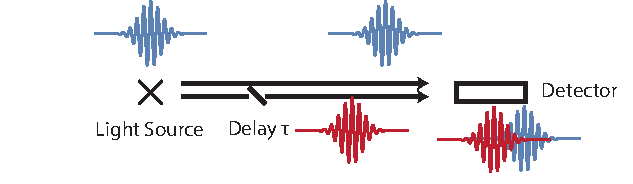
\includegraphics[width=0.8\linewidth]{images/michelson.pdf}
	\caption[Schematic of interferometer]{Schematic of interferometer: Light of (a gaussian) light source with finite coherence time is split and interference with a delayed copy is observed. The time averaged intensity measured by an detector changes with the delay time. }
	\label{fig:michelson}
\end{figure}

\begin{equation}
V=\left|g_1\right|
\end{equation}

Int
-along Glauber/Statistical Optics Goodman



Intensity in double slit leads to normalized degree of coherence $g_1$
Visiblity is modulus of $g_1$.

In a double slit setup (\fref{fig:doubleslit}), $E(r,t)=c_1 E_1(t)+c_2E2(t)$ with complex $c_2$ and $c_2$, $\left|c_1\right|\approx\left|c_2\right|$ describing the propagation to the screen. 

\begin{figure}
	\centering
	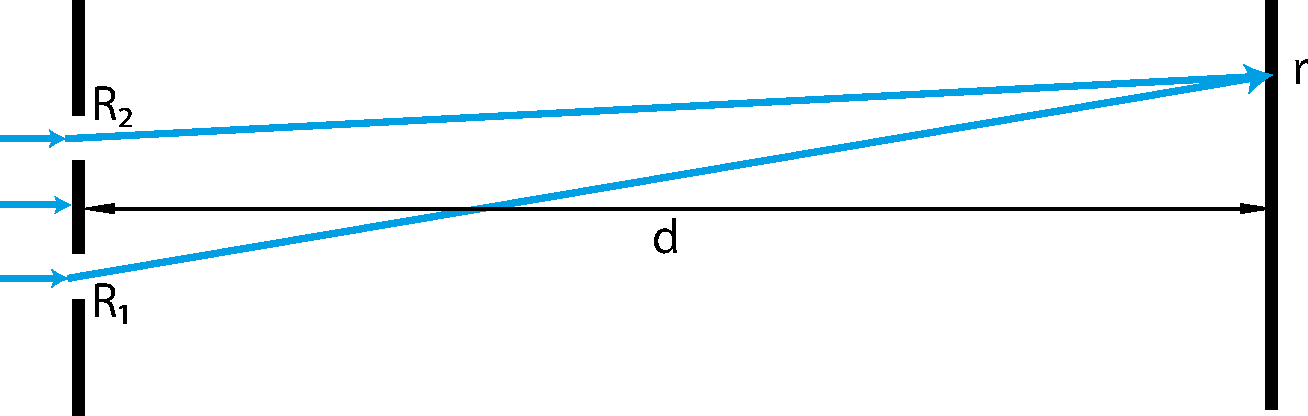
\includegraphics[width=0.8\linewidth]{images/doubleslit.pdf}
	\caption[Schematic of double slit]{Schematic of double slit: Monochromatic light goes through slits located at $R_1$ and $R_2$. The intensity at a position $r$ on the scree (in distance $d$) is the superposition of both paths.  If the slits are within the lateral coherence area of the source, the visibility of the interference pattern depends on the path length difference in comparison to the coherence time $\tau$.}
	\label{fig:doubleslit}
\end{figure}


\paragraph{Second order coherence $g_2(t_1,t_2)$}
The definition of $g_1$ can be extended to the second order by
\begin{equation*}
	g^{(2)}(\vec{r}_1,t_1;\vec{r}_2,t_2= 
	\frac{\left< E^*(\vec{r}_1,t_1)E^*(\vec{r}_2,t_2)E(\vec{r}_1,t_1)E(\vec{r}_2,t_2) \right>}{\left<\left | E(\vec{r}_1,t_1)\right |^2 \right> \left< \left |E(\vec{r}_2,t_2)\right |^2 \right>}	
\end{equation*}
For classical fields normalized correlations of intensities:
\begin{equation}
	g^{(2)}(\vec{r}_1,t_1;\vec{r}_2,t_2)= 
		\frac{\left< I(\vec{r}_1,t_1)I(\vec{r}_2,t_2 \right>}{\left<I(\vec{r}_1,t_1)\right>\left<I(\vec{r}_1,t_1)\right>}	
\end{equation}

\paragraph{Van Cittert Zernicke}
The Van Cittert–Zernike theorem establishes that in the far field, the coherence function of a 
quasi-monochromatic but spatially incoherent light source is proportional to the 2D Fourier transform intensity distribution of the source and Carter and Wolf introduced a generalization for three dimensional sources, showing that in the case of an completely incoherent source field, the complex degree of coherence is proportional to the 3D Fourier transform of the source's intensity distribution \cite{rosen1996, goodman200, carter1981}:
\begin{equation}
	g^{(1)}(\vec{r}_1,\vec{r}_2) \propto I_0^{-1} \int_{S} I_s(\vec{r}) \frac{e^{ik(R_1-R_2)}}{R_1 R_2} \difc \vec{r}
\end{equation}
with the source volume $S$ and intensity distribution $I_s$, total source intensity $I_0=\int I_s(\vec{r}) \difc \vec{r}$ and distances $R_{1,2}=\left|\vec{r}_{1,2}-\vec{r}\right|$. 
%-Hanbury Brown and Twist
\section{Hanburry Brown Twiss}
Hanburry Brown and Twiss 


\paragraph{Siegert Relation}
For thermal light, 
\begin{equation}
	g_2(\vec{r_1},\vec{r_2}) = 1+ |g_1(\vec{r_1},\vec{r_2}) |^2 ,
\end{equation}
which is called the Siegert Relation.
For $N$ Single-Photon-Emitters, a similiar form holds \cite{classen2017}:
\begin{equation}
	g_2(\vec{r_1},\vec{r_2}) = 1+ |g_1(\vec{r_1},\vec{r_2}) |^2 - \frac{2}{N} ,
\end{equation}
As, as according to the van Cittert Zernicke theorem \fref{eq:vcz}, $g_1$ encodes structural information, 
\begin{equation}
g_1(\vec{k_1},\vec{k_2}) \propto \mathscr{F}S(\vec{r}) = S(\vec{q})
\end{equation}
the difference of the intensity-intensity correlation from unity is proportional (with a contrast determining constant $\beta$) to the Fourier transform of the arrangement of emitters with $q=\vec{k_1}-\vec{k_2}$ (see \fref{fig:scatteringvectors}).
 \begin{figure}
	\centering
	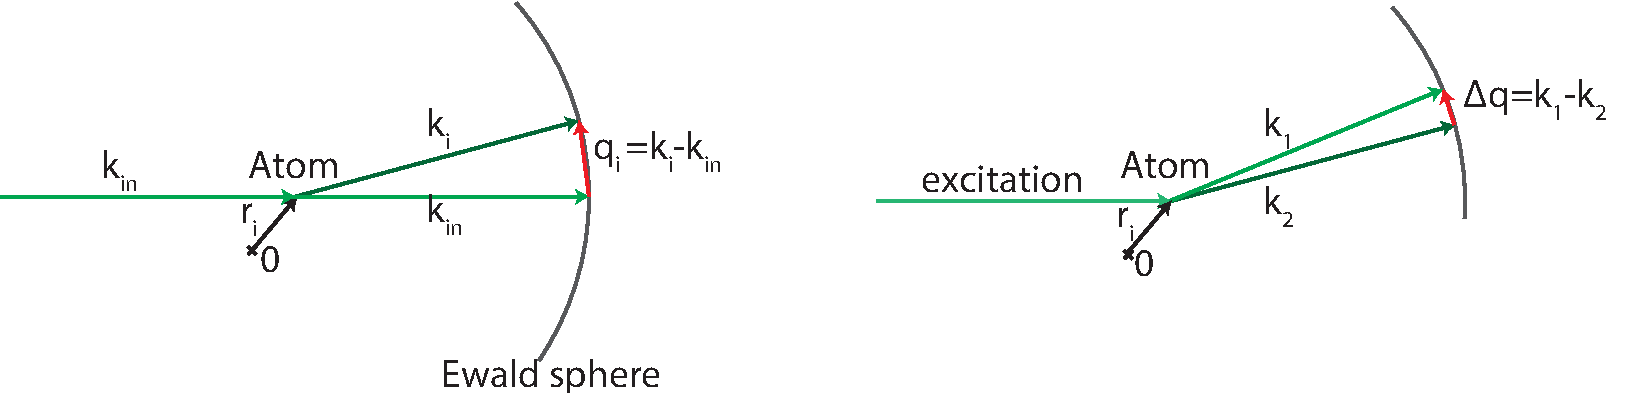
\includegraphics[width=0.9\linewidth]{images/scatteringvectors.pdf}
	\caption[Scattering Vectors]{Scattering vector $q$ in CDI (left) and IDI (right). In CDI, $q$ is the momentum transfer between incoming and outgoing wave. In IDI, there is no momentum transfer from the incoming to the outgoing wave. Instead, intensity correlations of different $k_1$, $k_2$ give a momentum transfer $\delta q$ according to the Siegert relation.}
	\label{fig:scatteringvectors}
	
\end{figure}

%-Single Photon Emitters/2nd Quant description
%(siehe Referenzen in Schaller/resonance fluorescence)
%-Fluorescence g2
%$2 Level with finite Lifetime -> Spectrum of fluorescence
\section{X-Ray Fluorescence}
 \begin{figure}
	\centering
	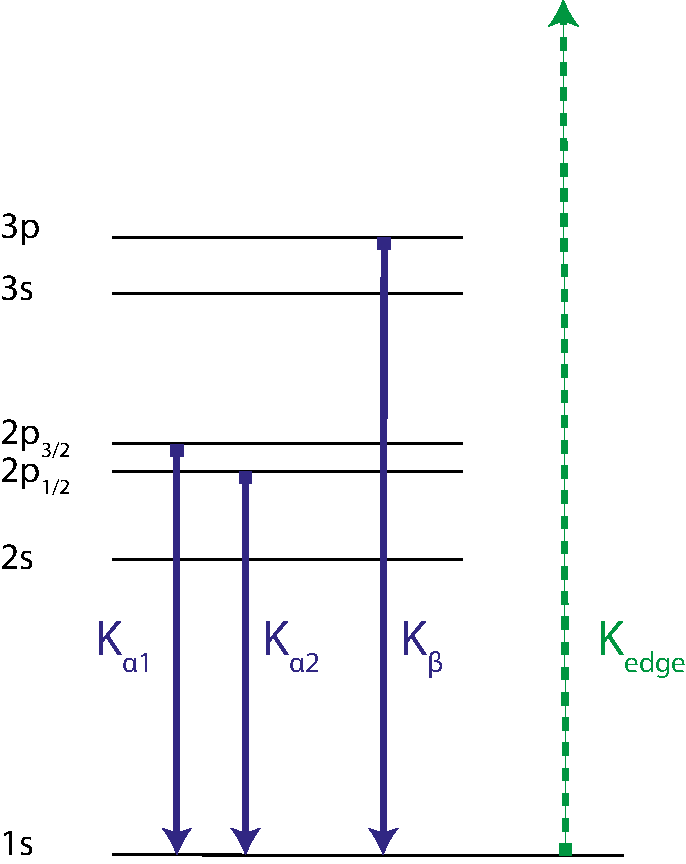
\includegraphics[width=0.4\linewidth]{images/levels.pdf}
	\caption[Atomic Levels]{Atomic levels and associated X-Ray energies}
	\label{fig:levels}
\end{figure}


\begin{table}[]
	\caption[X-Ray Energies]{X-Ray Energies of some relevant elements. }
	\small
	\begin{tabular}{l|l|ll|lll|ll}
		\hline
		Element & K$_{edge}$                                             & \multicolumn{2}{c}{K${_\alpha 1}$}                                                                           & \multicolumn{3}{c}{K${_\alpha 2}$}                                                                                                                                       & \multicolumn{2}{c}{K${_\beta 1,3}$}                                                                              \\
		& \begin{tabular}[c]{@{}l@{}}Energy \\ / eV\end{tabular} & \begin{tabular}[c]{@{}l@{}}Energy \\ / eV\end{tabular} & \begin{tabular}[c]{@{}l@{}}FWHM \\ / eV\end{tabular} & \begin{tabular}[c]{@{}l@{}}Energy\\  / eV\end{tabular} & \begin{tabular}[c]{@{}l@{}}FWHM \\ / eV\end{tabular} & \begin{tabular}[c]{@{}l@{}}rel. \\ Intensity\end{tabular} & \begin{tabular}[c]{@{}l@{}}Energy\\ / eV\end{tabular} & \begin{tabular}[c]{@{}l@{}}rel. \\ Intensity\end{tabular} \\ \hline
		Fe      & 7112                                                   & 6403.8                                                 & 1.61                                                 & 6390.8                                                 & 1.62                                                 & 0.50                                                      & 7058.0                                                & 0.17                                                      \\
		Cu      & 8979                                                   & 8,047.8                                                & 2.11                                                 & 8,027.8                                                & 2.17                                                 & 0.51                                                      & 8905.3                                                & 0.17                                                      \\
		Ga      & 10367                                                  & 9251.7                                                 & 2.59                                                 & 9224.8                                                 & 2.66                                                 & 0.51                                                      & 10263.9                                               & 0.71                                                      \\
		As      & 11867                                                  & 10543.7                                                & 3.08                                                 & 10508.0                                                & 3.17                                                 & 0.51                                                      & 11724.3                                               & 0.19                                                      \\ \hline
	\end{tabular}
\end{table}
\section{Intensity Correlations using X-Ray Fluorescence}
\section{Signal to Noise Considerations}


The noise in the measurement will consist of three parts: First, noise inherent to IDI caused by the random distribution of phases, second, the poissonian noise caused by quantized photons and third, meassurment noise caused by an imperfect detector.

Which factors influence SNR
-lifetime/pulsewidth
-polarisation
-sampling conditions / undersampling
-sample thickness / coherence length
-N images
-N photons



The speckle contrast $\beta$ is governed by the number of independent modes $M$ overlaid in the measurement \cite{goodman2000}.
\begin{equation}
\beta =\tfrac{1}{M}
\end{equation}

If the measurement is performed over a finite amount of time the number of temporal degrees of freedom is
\begin{equation}
M_t=\frac{\left(\int_{-\infty}^{\infty} P(t)\diff t\right)^2}{\int_{-\infty}^{\infty} K(t) \left|\mu(t)\right|^2\diff t}
\label{eq:modes}
\end{equation}
with $P(t)$ the integration window weighting function and $K(t)$ its autocorrelation \cite{goodman2007}. If the integration windows is set by the integration time $T$ of the detector, $P(t)$ is a rectangular function with the width $T$ and
\begin{align}
M_t,rect =T \left[\int_{-\infty}^{\infty} \Lambda\left(\frac{t}{T}\right) \left|\mu(t)\right|^2 \diff t \right]^{-1} .\\
\text{with  }\Lambda(x) = \begin{cases} 
 1-\left|x\right|& \textit{if }|x|<1\\
0 & \textit{otherwise}\\ 
\end{cases}
\label{eq:modesapprox}
\end{align}
Considering the case of a long integration time, $T\gg\tau$, this can be approximated as $M\approx\frac{T}{\tau}$. For a short integration time,  $T\ll\tau$, the number of temporal modes $M$ approaches unity.

If the Integration time can be considered as infinite and instead $P(t)$ is a Gaussian excitation pulse with FWHM of $\tau_p=2\sigma\sqrt{2\ln2}$ and unit area convoluted with an exponential decay with lifetime $\tau_d$ \cite{butz2015},
\begin{align}
P(t)&=\frac{1}{\tau_d\sigma\sqrt{2\pi}} \int_0^{\infty} e^{-\frac{t^{\prime}}{\tau_d}} 
e^{-\frac{(t-t^{\prime})^2}{2\sigma^2}}\diff t^{\prime}
=\frac{1}{2\tau_d}e^{-\frac{t}{\tau_d}+\frac{\sigma^2}{2\tau_d^2}}
\erfc\left[
\frac{\sigma}{\sqrt{2}\tau_d}
-\frac{t}{\sqrt{2}\sigma}
	\right] ,
	\label{eq:pfull}
	\end{align}
	with the complementary error function $\erfc=\frac{2}{\sqrt{\pi}}\int_x^\infty e^{-z^2}\diff z$ an approximation can be made if the pulse length is long in comparison the to coherence time, dropping the exponential decay from $P(t)$ and simplifying its autocorrelation to
\begin{align}
K(t)&\approx \sqrt{\frac{2{\ln 2}}{\pi}}\frac{1}{ \tau_p} e^{-\left(\sqrt{2\ln 2}\frac{t}{\tau_p}\right)^2} .
\end{align}
The number of degrees of freedom in this approximation is
\begin{align}
M_t,gauss&=\left[\int_{-\infty}^{\infty} K(t) \left|\mu(t)\right|^2\diff t\right]^{-1}.
\label{eq:modesapprox2}
\end{align}
For a Lorentzian spectrum (see \fref{eq:docdecay}), the numerical solution of \fref{eq:modes} and the approximations introduced in \fref{eq:modesapprox} and \fref{eq:modesapprox2} is shown in \fref{fig:modes} 
\footnote{To numerically evaluate \fref{eq:pfull} and integrals involving it, the introduction of the scaled error function $\text{erfcx}(x)=e^{x^2} \text{erfc}(x)$ and switching between using $erfc$ and an sufficient approximation for $erfcx$ depending on the parameters is necessary to avoid under- or overflow of the numerical representation of either the exponential or the error function term.}



The experimentally indistinguishable fluorescence energies $K_\alpha,1$ and $K_\alpha,2$ (as well as  $K_\beta$ if no filter is used for suppression) give additional independent modes $M_E$

As the used X-ray detectors are polarization insensitive and X-ray fluorescence is unpolarized and the incoherent field can be separated into two polarization modes, which are pairwise orthogonal with $\vec{k}$ and therefore change slightly for each atom and detector position. For small source dimensions, this change is negligible,  giving $M_P \approx 2$. 


Path differences longer than the coherence length give additional modes $M_S$, therefore the speckle visibility will be reduced for large samples:

If the speckle pattern is not spatially resolved by the detector because its resolution is to low compared to the change in intensity, undersampling will occur, the meassured signal will be spatially averaged giving independent sampling modes $M_D$





As an approximation, the total number of modes can be considered the product of those modes different numbers discussed above, even though in reality, the mode numbers are not completely independent.
Therefore, in \fref{chap:simulation}  simulations under different conditions with experimentally feasible  parameters will be performed.
%- SNR
%will use Peak/stdev bg definition


\label{chap:theory}


\section{Statistics}
Consider a complex sum of phasors of constant amplitude $A$ and independent uniformly in $(-\pi,\pi)$distributed phases $\phi_k$,
\begin{align}
c=\sum^N_k A e^{i\phi_k}
\end{align}
For sufficiently large numbers of $N$, the real and imaginary parts
\begin{align*}
r&=\Re c =  A \sum^N_k \cos(\phi_k)\\
i&= \Im c =A \sum^N_k \sin(\phi_k)
\end{align*}
will (by Central Limit Theorem) be Gaussian random variables with zero mean and variance $\sigma^2=\frac{N}{2}A^2$ and the probability distribution of the amplitude $a=\sqrt(a^2+i^2)$ will  therefore be the Rayleigh distribution
\begin{equation}
p(a)=\frac{1}{2\pi\sigma^2} a e^{\frac{a^2}{2\sigma^2}}
\end{equation}
and  $I=\left|a\right|^2$ will  follow an exponential distribution
\begin{equation}
\label{eq:expdistr}
p(I)=\frac{ e^{-I/\overline{I}}}{\overline{I}}
\end{equation} 
with mean $\overline{I}$ and standard deviation $\sigma=\overline{I}$  \cite{goodman2000,goodman1976}.
A sum of $M$ uncorrelated random variables following identical distributions given by \fref{eq:expdistr} follows a Gamma distribution,
\begin{equation}
\label{eq:gammadistr}
p(I)=\frac{I^{M-1} e^{-I/\overline{I}}} {\overline{I}^M \Gamma(M)},
\end{equation}
for a positive integer $M$ this simplifies with $\Gamma(M)=(M-1)!$ to an Erlang distribution  \cite{forbes2010,trost2020}.
If $I$ is distributed like \fref{eq:gammadistr} and furthermore Poisson sampled as discrete $k$ (such as photon counts), it follows  an negative binomial distribution,
\cite{trost2020,mandel1959,holmes2019}
\begin{equation}
p(k)=
\frac{\Gamma(k+M)}{\Gamma(M)\Gamma(k+1) }
\left( 1+\frac{1}{\overline{I}}
\right)^{-k}
\left( 1+\overline{I}
\right)^{-M}
\end{equation}
with mean $\mu=M\overline{I}$ and variance $\mu+\frac{\mu^2}{M}$ (which differs from the variance of a poisson distribution $\mu$).

This probability distribution can be compared to an experimental measured photon count distribution and the number of modes present in the measurement can be estimated by a regression \cite{lehmkuhler2014,yun2019}.

The variance of a product of (uncorrelated) photon counts  following this distribution will have a variance of
\begin{equation}
\Var_{p\cdot p}= \Var_p^2 +2 \mu^2\Var_p	= \mu^4 \frac{2 M + 1}{M^2 + 2}+ \mu^3 \frac{M+1}{M} + \mu^2 \,.
\end{equation}

Following the idea of Trost et. al, this can be used so estimate the noise of an intensity correlation measurement, even though the actual signal will break the assumption of having uncorrelated photon counts \cite{trost2020}.
\begin{figure}
\centering
\includegraphics[width=0.6\linewidth]{images/modes.pdf}
\caption[Photon Statistics with different numbers of Modes]{Photon statistics with different numbers of modes $M$ and equal mean of 0.1\,photons. A lower number of modes corresponds the an higher probability of observing multi photon events. The limit of a high number of modes is a Poisson distribution.}
\end{figure}
\section{Kossel Lines}
X-Ray radiation originating from within a single crystal gets Bragg reflected at the lattice planes, causing Intensity variation in $90^o-\theta$ around the direction $k_{hkl}$, forming the \textit{Kossel Cones}. On the spherical detector centered at at the crystal, the points with influenced intensity would lie on circles with radii determined by ...

The visibility of the Kossel lines is governed by the same extinction rules as for the Bragg reflexes for, the structure factor $F_{hkl}$ has to be non-zero. For a zinc blende structure (such as GaAs) with atomic scattering factors $f_a$ and $f_b$, the structure factor is
\begin{align}
F_{hkl} = \begin{cases}
0, & \text{if $h$, $k$, $l$ mixed parity}.\\
4(f_a+f_b), & \text{if same parity and $h+k+l = 4 N$} \\
4(f_a\pm i f_b), & \text{if same parity and $h+k+l = 2 N+1$} \\
4(f_a-f_b), & \text{if same parity and $h+k+l = 4 N+2$} \\
\end{cases}
\end{align}

The structure of the intensity variations (both intense and less intense depends on the which case...
If the fine structure cannot be resolved

The Kossel lines allow to orient the detector with regards to the lattice planes. This can either be done by reprojecting the planar detector onto a sphere by an inverse gnomonic projection and determining circle center and radius, eg. by an Hugh-Transform, or by a fitting conic sections to the lines on the planar detector. As the observable curvature of the Kossel lines on the detector in an IDI setup is small and therefore the circles are difficult to determine, the second method will be used. 

As each point identifyed as beloning to a Kossel line has to be part of a conic section of the same plane with each cone originating from the same point, each point $r$ on a line has to fullfill



\begin{equation}
\frac{\vec{r} \cdot \vec{q}}{\left|\vec{r}\right| \left| \vec{q}\right|} = \frac{\lambda}{2d}
\end{equation}
 for a reciprocal lattice vector $q$ which is an element of the allow reflections $Q$. So finding the dector orientation can be seen as finding a rotation Matrix $R$ as
\begin{equation}
\arg\!\min_{R} \sum_{r} \min_{q\in Q} \frac{2 d * \vec{r} \cdot \vec{Rq}}{\left|\vec{r}\right| \left| \vec{q}\right|} -\lambda
\end{equation}
\begin{figure}
	\centering
	\begin{subfigure}[b]{0.25\textwidth}
	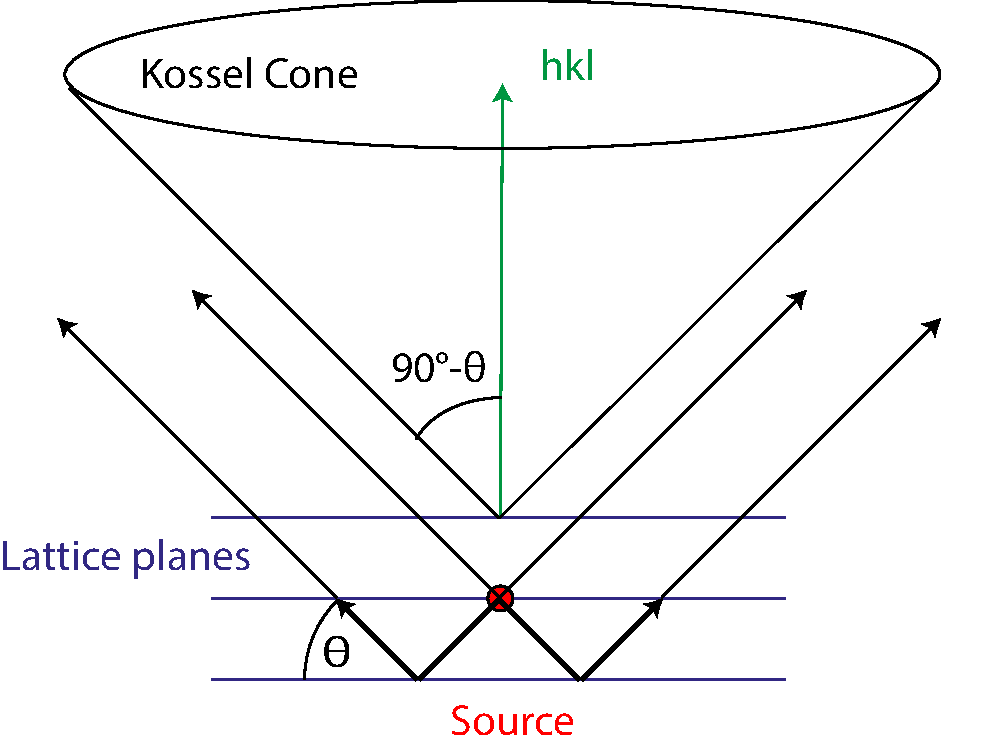
\includegraphics[width=\linewidth]{images/kossel0.pdf}
	\end{subfigure}
	\begin{subfigure}[b]{0.25\textwidth}
	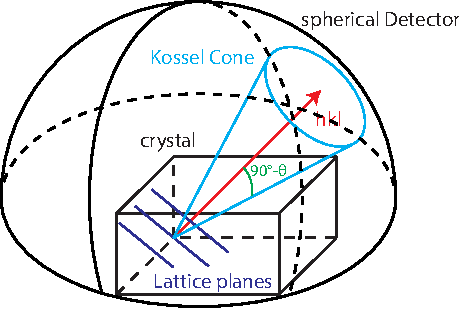
\includegraphics[width=\linewidth]{images/kossel.pdf}
	\end{subfigure}
	\begin{subfigure}[b]{0.35\textwidth}
	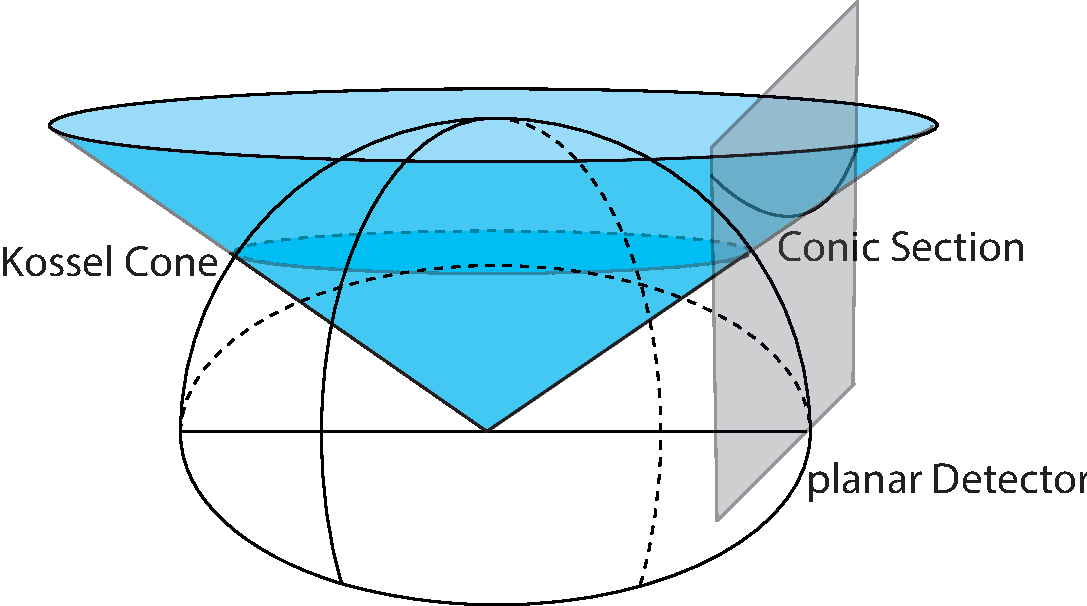
\includegraphics[width=\linewidth]{images/kossel2.pdf}
	\end{subfigure}
	\caption[Geometry of Kossel Lines]{Geometry of Kossel Lines: Radiation from within a light source within a single crystal gets scattered at the lattice planes, causing a change in intensity along a cone of opening angle $90^o-\theta_{hkl}$ and vertex hkl (left). On a spherical detector centered around the sample, those intensity changes would be visible as circular Kossel lines (center). On a planar detector, the intersections of the Kossel cones are visible as conic sections (right)}
	\label{fig:doubleslit}
\end{figure}